\chapter*{Autoras e Autores}
\begin{wrapfigure}{l}{0pt}
    
\includegraphics[width=0.2\paperwidth]{autoras/amandamorais.jpg}
\end{wrapfigure}

\noindent Amanda Oliveira de Morais é docente na Universidade Estadual de Londrina, mestra em Análise do Comportamento pela Universidade Estadual de Londrina (UEL), graduada em psicologia pela Universidade Estadual de Londrina, membra e fundadora do Coletivo Marias \& Amélias de Mulheres Analistas do Comportamento e psicóloga clínica. Também foi docente da Universidade Estadual de Maringá (UEM).\\
\linebreak
\linebreak
\begin{wrapfigure}{l}{0pt}
    \centering
    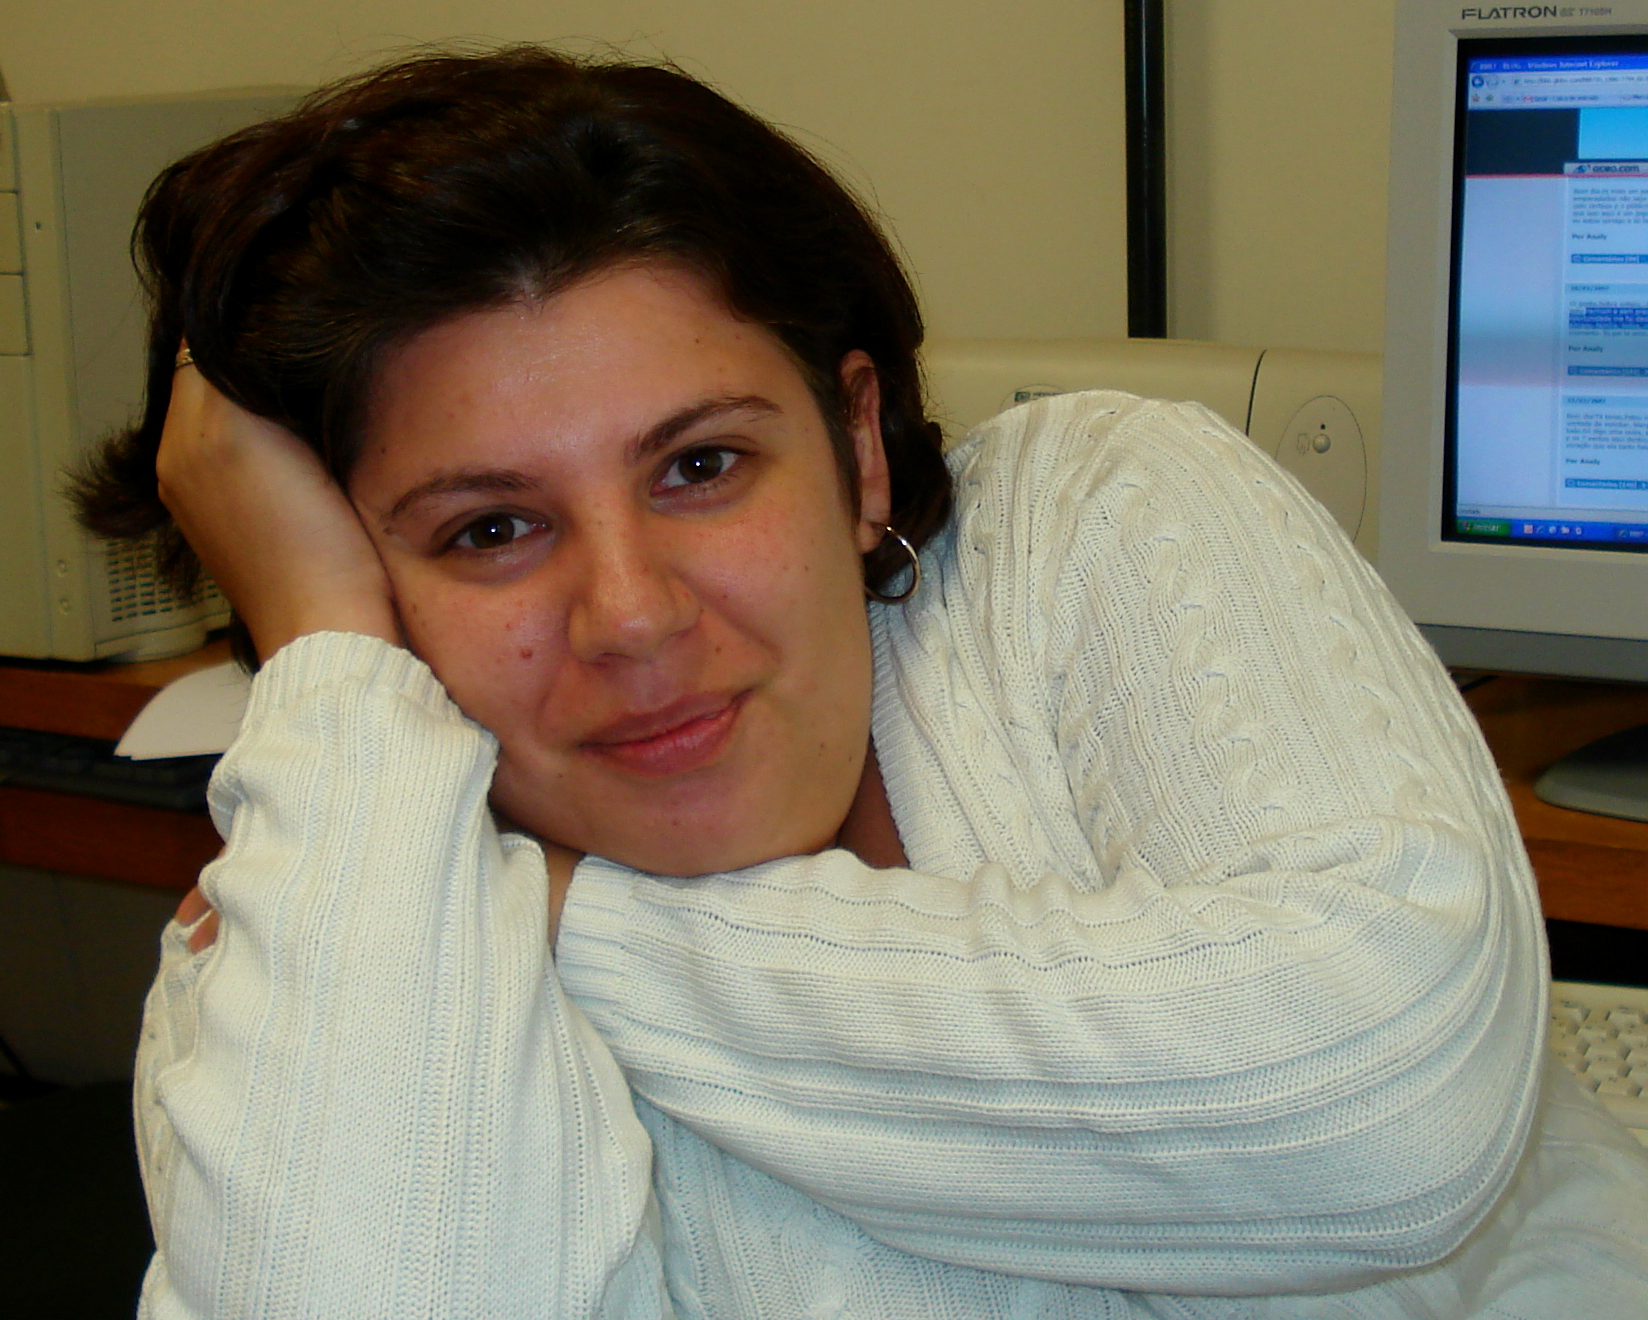
\includegraphics[width=0.2\paperwidth]{autoras/anaarantes.jpg}
\end{wrapfigure}

\noindent Ana Arantes é pesquisadora de Pós-doutorado no Laboratório de Aprendizagem Humana, Multimídia Interativa e Ensino Informatizado (LAHMIEI), docente e pesquisadora associada do Departamento de Psicologia da Universidade Federal de São Carlos (UFSCar). Desenvolve pesquisas experimentais e teórico-conceituais na área de comportamento social, investigando fenômenos comportamentais ligados à temática do feminismo e das opressões sistemáticas de gênero e raça. É membra fundadora do Coletivo Feminista Marias \& Amélias de Mulheres Analistas do Comportamento e líder do Grupo de Pesquisa e Análise Comportamental das Práticas Culturais de Opressão de Gênero e Raça. Divulgadora científica do ScienceBlogs Brasil e autora do blog O Divã de Einstein, além de ser consultora dos canais Nerdologia e Minutos Psíquicos no Youtube e participante do Time de Ciências do podcast Nerdcast.